\subsection{Diagrammes}

\subsubsection{Diagramme de cas d'utilisation :}

\begin{center}
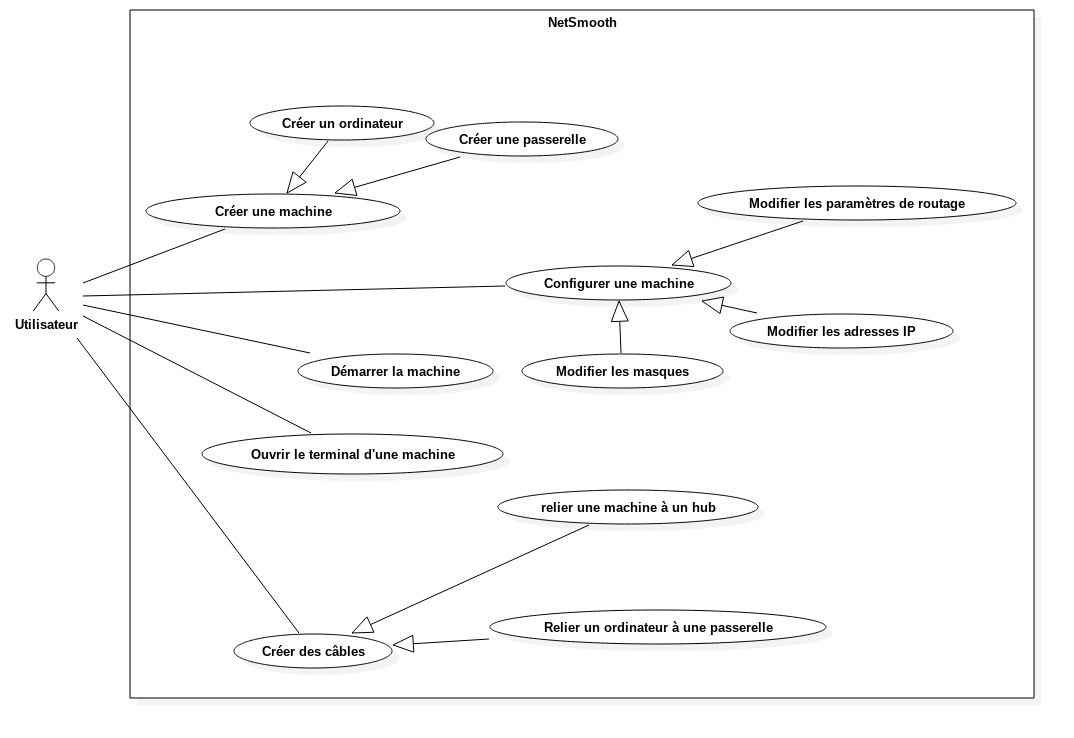
\includegraphics[scale=0.47]{usecase_diagram.png}
\end{center}

\newpage
\subsubsection{Diagramme de classe d'analyse}
\begin{center}
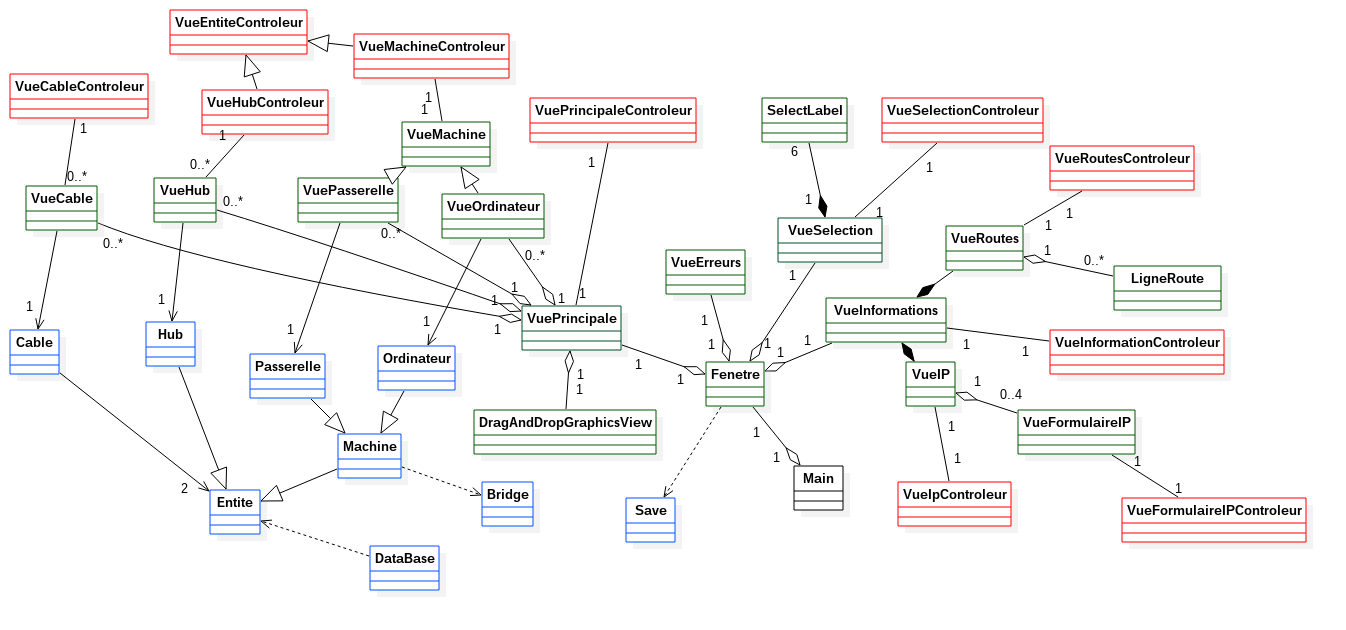
\includegraphics[scale=0.5]{diagramme_analyse.png}
\end{center}

Les classes en rouge représentent les contrôleurs, les classe en vert les vues, puis les classes en bleu les modèles.

\newpage
\subsection{Diagrammes de séquence}
\textbf{Créer une machine, un hub ou une passerelle - première version}
\begin{center}
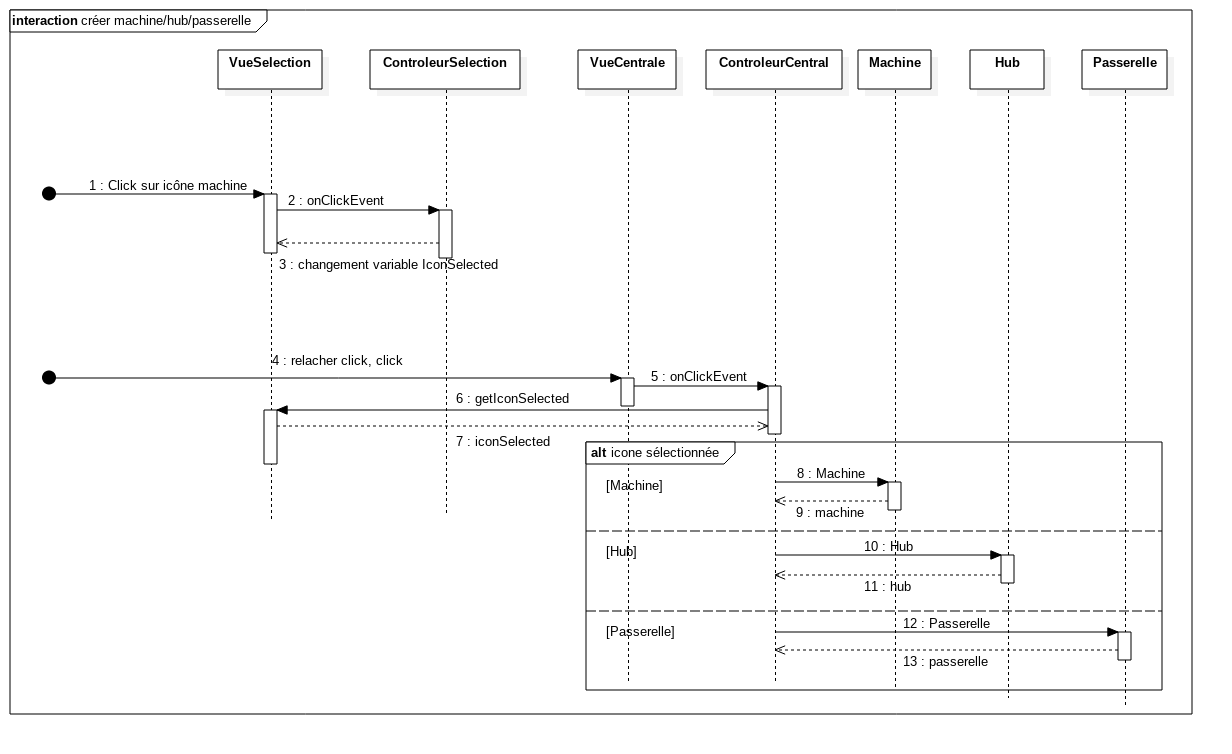
\includegraphics[scale=0.4]{createmachine.png}
\end{center}

\textbf{Démarrer une machine ou une passerelle} 
\begin{center}
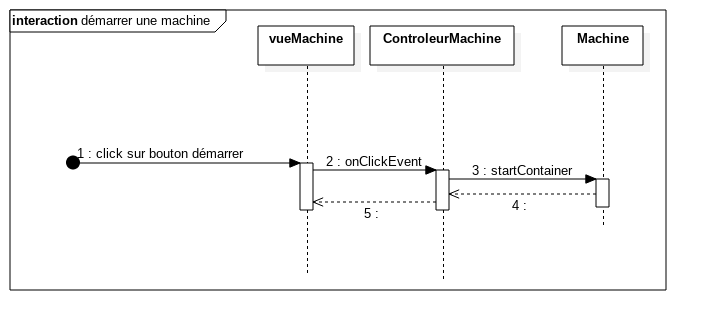
\includegraphics[scale=0.55]{startmachine.png}
\end{center}

\vspace{17\baselineskip}
\textbf{Configurer une machine/passerelle éteinte} 
\begin{center}
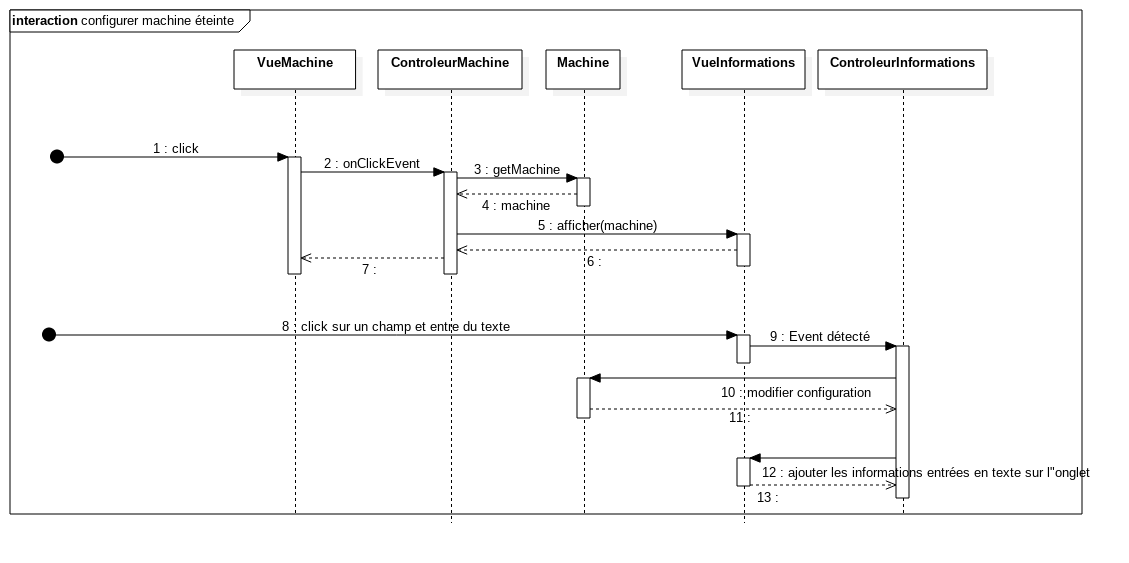
\includegraphics[scale=0.4]{configuredownmachine.png}
\end{center}

\textbf{Ouvrir terminal d'une machine allumée} 
\begin{center}
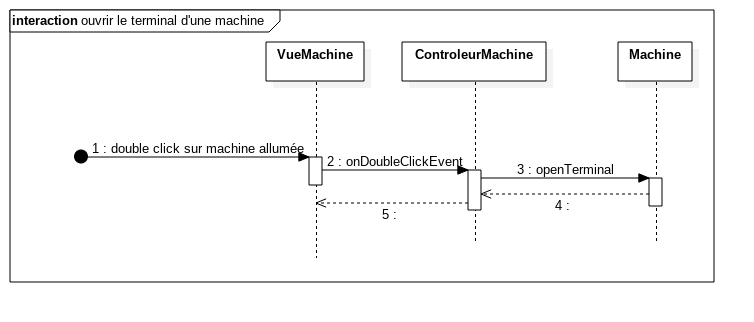
\includegraphics[scale=0.6]{openterminal.png}
\end{center}

\vspace{16\baselineskip}
\textbf{Créer un cable} 
\begin{center}
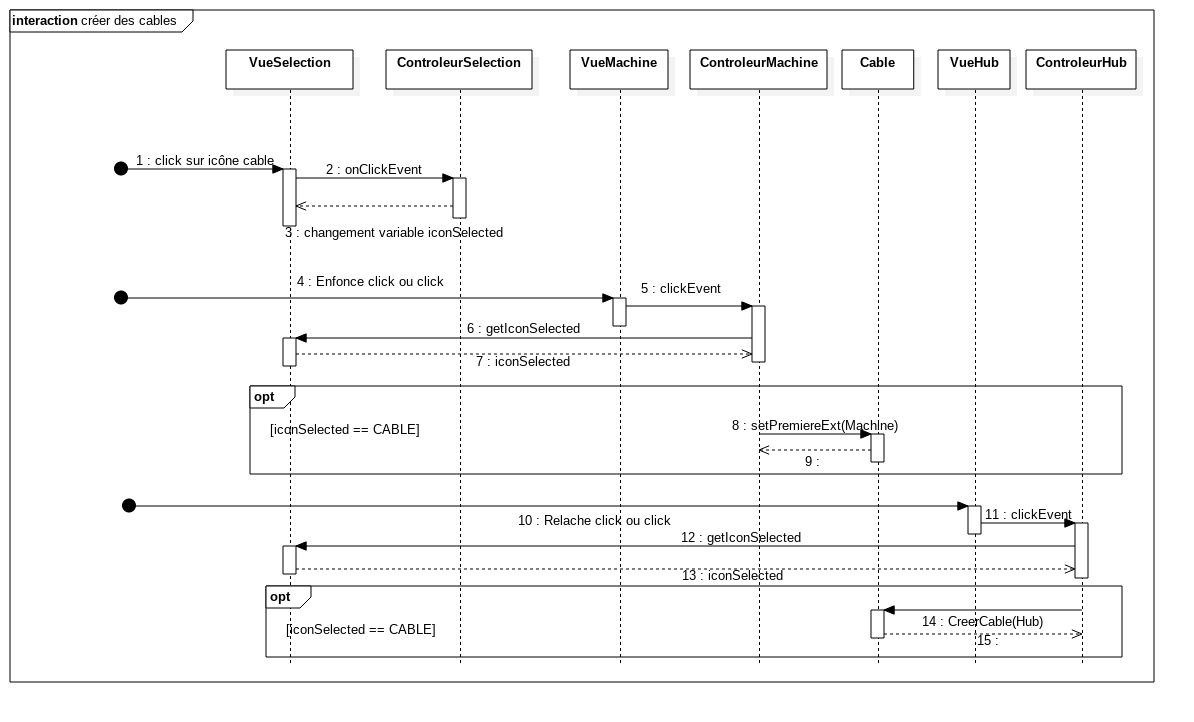
\includegraphics[scale=0.4]{createcables.png}
\end{center}
\newpage